% ======================================================================
%  Chapter 9 — The Microwave Photonic Crystal  (EXPANDED)
% ======================================================================

\section{From theory to the laboratory}
\label{sec:ch9-intro}

The preceding three chapters developed the theory of photonic Chern
insulators: Dirac cones from lattice symmetry, their gapping by
magneto-optical perturbation, and the one-way interface mode that
necessarily threads the resulting topological gap.  But the theory would
remain an elegant analogy were it not for a remarkable experiment.

In 2009, Wang, Chong, Joannopoulos, and Solja\v{c}i\'{c} demonstrated
unidirectional electromagnetic edge transport in a two-dimensional
gyromagnetic photonic crystal operating in the microwave regime
\cite{nature2026observation}.  Their experiment achieved a
forward-to-backward transmission ratio exceeding $10^5$, providing the
first direct observation of a photonic analog of the quantum Hall edge
state.  This chapter describes the experiment in detail: the material
choice, the crystal design, the measurement geometry, and the
quantitative comparison with the predictions of Chapters~7 and~8.

The experiment was preceded by a theoretical proposal in 2008
\cite{haldane2008possible}, in which Haldane and Raghu showed that
photonic Dirac points in a gyromagnetic crystal can be gapped by a
magneto-optical perturbation, producing bands with nonzero Chern
numbers and hence one-way edge modes
\cite{raghu2008analogs}.  A companion paper by Wang,
Chong, Joannopoulos, and Solja\v{c}i\'{c} (2008) computed the
complete band structure of a specific YIG rod lattice, predicted the
existence of one-way edge states in a particular frequency window, and
proposed the parallel-plate waveguide geometry that was subsequently
realised experimentally \cite{ozawa2018topological,wang2015topological}.  The experiment
thus confirmed a precise, first-principles prediction rather than an
accidental discovery.

\section{Material platform: yttrium iron garnet}
\label{sec:ch9-yig}

\subsection{Why ferrites at microwave frequencies}
\label{sec:ch9-why-ferrites}

The theory of Chapter~7 requires a material whose permeability tensor
has a nonzero off-diagonal (gyrotropic) component $\kappa_\mu$
\cite{haldane2008reflection}.  At
optical frequencies, magneto-optical effects exist in semiconductor and
rare-earth materials, but they are weak: the Verdet constant of
bismuth iron garnet, one of the strongest Faraday-active optical
materials, produces rotation of order $10^3\;\mathrm{deg/cm}$---still
far too small to open a topological gap in a photonic crystal of
reasonable size.

At microwave frequencies, the situation is qualitatively different.
Magnetised ferrites support ferromagnetic resonance (FMR), and near
the FMR frequency the off-diagonal permeability $\kappa_\mu$ becomes
of order unity.  The key material is yttrium iron garnet
($\mathrm{Y_3Fe_5O_{12}}$, YIG), which combines large gyromagnetic
response with extremely low magnetic loss.

\subsection{The Polder permeability of YIG}
\label{sec:ch9-polder}

As derived in Appendix~D, the permeability tensor of a saturated ferrite
magnetised along $\hat{z}$ has the Polder form
\cite{gangaraj2016berry,he2016photonic}
\begin{equation}\label{eq:ch9-polder}
  \mut = \begin{pmatrix}
    \mu_\perp & -\ii\kappa_\mu & 0 \\
    \ii\kappa_\mu & \mu_\perp & 0 \\
    0 & 0 & 1
  \end{pmatrix},
\end{equation}
with
\begin{equation}\label{eq:ch9-polder-params}
  \mu_\perp(\omega) = 1 + \frac{\omega_0\omega_m}{\omega_0^2 - \omega^2}\,,
  \qquad
  \kappa_\mu(\omega) = \frac{\omega\omega_m}{\omega_0^2 - \omega^2}\,.
\end{equation}
The Larmor frequency $\omega_0=\gamma B_0$ is set by the applied bias
field $B_0$, and the magnetisation frequency
$\omega_m=\gamma\mu_0 M_s$ is set by the saturation magnetisation
$M_s$.  For YIG the gyromagnetic ratio is
$\gamma/(2\pi)\approx 28\;\mathrm{GHz/T}$ and the saturation
magnetisation gives $\omega_m/(2\pi)\approx 4.9\;\mathrm{GHz}$.

At frequencies below ferromagnetic resonance ($\omega<\omega_0$), both
$\mu_\perp$ and $\kappa_\mu$ are positive and can be large.  The ratio
$\kappa_\mu/\mu_\perp$ determines the strength of time-reversal
breaking and hence the width of the topological gap.  For the Wang
experiment, parameters were chosen so that $\kappa_\mu/\mu_\perp$ is
of order $0.3$--$0.5$ in the operating band.

\subsection{Loss and linewidth}
\label{sec:ch9-loss}

YIG is exceptional among magnetic materials for its narrow
ferromagnetic resonance linewidth $\Delta H$.  Single-crystal YIG has
$\Delta H\lesssim 0.3\;\mathrm{Oe}$, corresponding to a magnetic
quality factor $Q_m=\omega_0/(2\gamma\mu_0\Delta H)\sim 10^4$.  This
means the imaginary parts of $\mu_\perp$ and $\kappa_\mu$ are negligible
over most of the frequency range below FMR, justifying the lossless
Hermitian treatment used in the topological theory.

Away from resonance, the magnetic loss tangent is typically
$\imag\mu/\real\mu < 10^{-4}$, so the mode decay over tens of lattice
constants is negligible.  This is essential: the topological edge mode
must propagate around the entire boundary of the crystal without
significant absorption.

\section{Crystal design}
\label{sec:ch9-crystal}

\subsection{Geometry}
\label{sec:ch9-geometry}

Wang et~al.\ used a square-lattice photonic crystal of YIG rods in air.
The rods are cylinders of radius $r=0.11a$ (where $a$ is the lattice
constant) with relative permittivity $\varepsilon_r=15$ and the Polder
permeability \eqref{eq:ch9-polder}.

The lattice constant was chosen so that the second and third TM bands
touch at a Dirac-like point near 4.5\;GHz.  The bias field
$B_0\approx 0.20\;\mathrm{T}$ (corresponding to
$\omega_0/(2\pi)\approx 5.6\;\mathrm{GHz}$) places the operating
frequency below ferromagnetic resonance, where the gyrotropic response
is strong but losses are minimal.

\subsection{Band structure}
\label{sec:ch9-bands}

The TM band structure of the square-lattice YIG crystal was computed
using the plane-wave expansion method described in
Chapter~\ref{ch:computing-chern}.  Without the applied magnetic field
($B_0=0$, $\kappa_\mu=0$), the second and third bands touch at a
doubly degenerate point on the $\Gamma$--$X$ line.  This degeneracy
is protected by time-reversal plus a mirror symmetry of the square
lattice.

When the field is applied ($B_0=0.20\;\mathrm{T}$), the gyrotropic
perturbation breaks time-reversal symmetry and opens a gap.  The gap
width is $\Delta\omega/(2\pi)\approx 0.12\;\mathrm{GHz}$, centred at
$\omega/(2\pi)\approx 4.5\;\mathrm{GHz}$.  The Chern numbers of the
bands below and above the gap are $\Chern_2=+1$ and $\Chern_3=-1$,
computed using the plaquette algorithm on a $20\times 20$ Brillouin-zone
grid with the electromagnetic inner product.

\subsection{Edge-state dispersion}
\label{sec:ch9-edge-dispersion}

The edge states were computed using a supercell geometry: a ribbon of
$N=20$ unit cells in the $x$-direction, periodic in $y$, with a metal
wall on one side and vacuum on the other.  The resulting projected band
structure shows a single branch crossing the topological gap, with
positive group velocity $v_g>0$ for all $k_y$ within the gap.  This
confirms that the edge mode is unidirectional: it propagates in the
$+y$ direction along the metal wall and cannot propagate backward.

\section{Experimental setup}
\label{sec:ch9-setup}

\subsection{Sample fabrication}
\label{sec:ch9-fabrication}

The photonic crystal was assembled by inserting single-crystal YIG rods
into a parallel-plate waveguide.  The rods were machined to a diameter
of $2r=2.2\;\mathrm{mm}$ and a height equal to the plate separation
($h\approx 7\;\mathrm{mm}$), ensuring that the fundamental TM mode
(with $E_z$ polarisation) is the only propagating mode in the frequency
range of interest.  The lattice constant was $a=10\;\mathrm{mm}$,
giving a ratio $r/a=0.11$.

A uniform magnetic bias field was provided by a pair of NdFeB permanent
magnets above and below the waveguide, producing $B_0\approx 0.20\;\mathrm{T}$
over the entire crystal area.

\subsection{Measurement geometry}
\label{sec:ch9-measurement}

Two coaxial probes, inserted through the top plate, served as source and
detector.  The source probe was placed at the edge of the crystal
(adjacent to the metal boundary), and the detector probe was scanned
along the edge in both the forward ($+y$) and backward ($-y$)
directions.  Transmission spectra were measured using a vector network
analyser over the frequency range 3.5--5.5\;GHz.

To test the robustness of the edge mode, a large metallic obstacle
(a cylinder of diameter $4a=40\;\mathrm{mm}$) was placed directly in
the path of the edge mode.  In a conventional waveguide, such an
obstacle would cause near-total reflection.

\section{Results}
\label{sec:ch9-results}

\subsection{Unidirectional transmission}
\label{sec:ch9-unidirectional}

The key result of the experiment is a dramatic asymmetry between
forward and backward transmission.  Within the topological gap
(4.45--4.57\;GHz), the forward transmission ($S_{21}$) was of order
$-10\;\mathrm{dB}$ (limited primarily by probe coupling loss), while
the backward transmission ($S_{12}$) was below the noise floor of the
network analyser at $-50\;\mathrm{dB}$.  This gives a forward-to-backward
ratio exceeding $10^4$ (conservatively), consistent with the theoretical
prediction of a single one-way edge mode.

Outside the topological gap, both forward and backward transmission
recover, as expected: the edge mode only exists within the gap.

\subsection{Robustness to obstacles}
\label{sec:ch9-robustness}

When the metallic obstacle was inserted in the edge-mode path, the
forward transmission decreased by less than 2\;dB.  The edge mode
simply routed around the obstacle, following the new boundary between
the photonic crystal and the metal.  No backward-scattered signal was
detected above the noise floor.

This result directly confirms the topological protection mechanism
described in Chapter~8: the one-way edge mode has no backward-propagating
partner at the same frequency, so there is no channel for
backscattering.  The mode can be forced to detour around an obstacle,
but it cannot reverse direction.

\subsection{Comparison with theory}
\label{sec:ch9-comparison}

The measured transmission spectra agree quantitatively with
finite-element simulations of the same geometry
\cite{ozawa2018topological}.  The gap frequency
range, the edge-mode group velocity, and the field profile at the
boundary all match the predictions of the plane-wave expansion
band structure computed with the Polder permeability.

One quantitative discrepancy is the absolute transmission level: the
measured forward transmission ($-10\;\mathrm{dB}$) is lower than the
simulated value ($-3\;\mathrm{dB}$), primarily due to impedance
mismatch at the coaxial probe tips.  This is an engineering issue
rather than a physics limitation, and subsequent experiments with
improved coupling have achieved forward transmission approaching
$-1\;\mathrm{dB}$.

\section{Significance and limitations}
\label{sec:ch9-significance}

\subsection{What the experiment demonstrates}
\label{sec:ch9-demonstrates}

The Wang experiment establishes three key facts about topological
photonic crystals \cite{nature2026observation,haldane2008possible}.  First, the theoretical prediction of one-way edge
modes based on Chern numbers and the bulk-edge correspondence is
confirmed quantitatively.  Second, the topological protection against
backscattering is real and dramatic: a large metallic obstacle causes
negligible reflection.  Third, the magneto-optical mechanism proposed by
Haldane and Raghu works in practice with commercially available ferrite
materials.

\subsection{Limitations of the microwave platform}
\label{sec:ch9-limitations}

The experiment operates at microwave frequencies ($\sim 4.5\;\mathrm{GHz}$,
wavelength $\sim 7\;\mathrm{cm}$), far from optical frequencies.
Scaling the effect to optical wavelengths faces two obstacles.

The first obstacle is material: magneto-optical effects at optical
frequencies are much weaker than at microwave frequencies.  The
gyrotropic parameter $\kappa_\mu/\mu_\perp$ of YIG at microwave
frequencies is of order $0.3$--$0.5$, but the corresponding Faraday
rotation in optical materials is orders of magnitude smaller per
wavelength.  Opening a topological gap large enough to accommodate an
edge mode at optical frequencies requires a different mechanism (such as
the reciprocal designs of Chapter~\ref{ch:reciprocal-designs} or the
Floquet modulation of Chapter~\ref{ch:floquet}).

The second obstacle is size: the photonic crystal has a lattice constant
comparable to the operating wavelength ($a\sim\lambda$), so a microwave
crystal with $a=10\;\mathrm{mm}$ is a tabletop experiment, while an
optical crystal with $a\sim 500\;\mathrm{nm}$ requires nanofabrication.
This is not a fundamental limitation, but it changes the experimental
difficulty and the potential applications.

\subsection{Subsequent experiments}
\label{sec:ch9-subsequent}

Following the Wang experiment, several groups have extended the result
in important ways \cite{ozawa2018topological,price2022roadmap}.  Larger crystals with more unit cells have confirmed
edge transport over longer distances.  Modified geometries have
demonstrated corner-turning without backscattering.  And perhaps most
importantly, the same topological physics has been demonstrated at
optical frequencies using different symmetry-breaking mechanisms
(Chapters~\ref{ch:reciprocal-designs}--\ref{ch:floquet}), confirming
that the Wang experiment was the beginning of a broad and versatile
field.

\section{Quantitative analysis of the topological gap}
\label{sec:ch9-gap-analysis}

It is instructive to trace the topological gap quantitatively from the
material parameters to the measured transmission spectrum, since this
chain of reasoning illustrates the power of the Maxwell-first approach.

\subsection{From Polder parameters to Dirac mass}
\label{sec:ch9-polder-to-mass}

At the operating frequency $\omega/(2\pi)=4.5\;\mathrm{GHz}$ with
$\omega_0/(2\pi)=5.6\;\mathrm{GHz}$ and
$\omega_m/(2\pi)=4.9\;\mathrm{GHz}$, the Polder parameters
\eqref{eq:ch9-polder-params} evaluate to
\begin{equation}\label{eq:ch9-polder-numerical}
  \mu_\perp \approx 1+\frac{5.6\times4.9}{5.6^2-4.5^2}
  \approx 3.47\,,
  \qquad
  \kappa_\mu \approx \frac{4.5\times4.9}{5.6^2-4.5^2}
  \approx 1.98\,.
\end{equation}
The gyrotropic ratio is $\kappa_\mu/\mu_\perp\approx 0.57$,
confirming that time-reversal breaking is strong.

In the language of the effective Dirac Hamiltonian
(\chref{ch:breaking-tr}), the gyrotropic perturbation produces a mass
term
\begin{equation}\label{eq:ch9-mass-estimate}
  \kappa
  \propto \kappa_\mu\,|\langle u_+|\hat{z}\cdot\nabla\times|u_-\rangle|
\end{equation}
at the band-touching point, where $|u_\pm\rangle$ are the two
degenerate Bloch modes.  The proportionality constant depends on the
field overlap integrals, which must be computed numerically for the
specific rod geometry; the plane-wave expansion of
\chref{ch:computing-chern} gives $\kappa/(2\pi)\approx 0.06\;\mathrm{GHz}$
for the Wang parameters, so the topological gap is
$\Delta\omega=2|\kappa|\approx 0.12\;\mathrm{GHz}$.

\subsection{From Chern number to edge-state count}
\label{sec:ch9-chern-to-edge}

The plaquette algorithm applied to the bands below and above the gap
yields $\Chern_2=+1$ and $\Chern_3=-1$.
The bulk-edge correspondence (\chref{ch:one-way-interface}) then
predicts exactly one chiral edge mode per edge of the crystal in this
gap.  This is consistent with the single branch observed in the
supercell edge-dispersion calculation and, crucially, with the
measured unidirectional transmission.

The quantitative chain is therefore:
\[
  \underbrace{B_0\;\to\;\omega_0,\omega_m}_{\text{material}}
  \;\to\;
  \underbrace{\mu_\perp,\,\kappa_\mu}_{\text{Polder}}
  \;\to\;
  \underbrace{\kappa}_{\text{Dirac mass}}
  \;\to\;
  \underbrace{\Chern=\pm 1}_{\text{topology}}
  \;\to\;
  \underbrace{\text{1 edge mode}}_{\text{experiment}}.
\]
Every step in this chain is computable from first principles, using
only Maxwell's equations and the constitutive parameters of YIG.  No
electronic analogy or tight-binding model is invoked.

\section{Eigenvalues of the Polder tensor}
\label{sec:ch9-polder-eigenvalues}

The gyrotropic permeability \eqref{eq:ch9-polder} has a rich
eigenvalue structure that directly controls the topological gap.
Because the off-diagonal blocks couple the $x$ and $y$ components
while leaving $z$ unchanged, we analyse the $2\times 2$ transverse
block
\begin{equation}\label{eq:ch9-mu-transverse}
  \mut_\perp = \begin{pmatrix}
    \mu_\perp & -\ii\kappa_\mu \\
    \ii\kappa_\mu & \mu_\perp
  \end{pmatrix}.
\end{equation}
The eigenvalues are found by diagonalising in the circular-polarisation
basis $\hat{e}_\pm=(\hat{x}\pm\ii\hat{y})/\sqrt{2}$:
\begin{equation}\label{eq:ch9-mu-eigenvalues}
  \mu_\pm = \mu_\perp \mp \kappa_\mu\,.
\end{equation}
The right-circular ($+$) and left-circular ($-$) polarisations
therefore propagate with different effective permeabilities.  The
splitting $\mu_+-\mu_-=-2\kappa_\mu$ is the permeability-space
measure of time-reversal breaking.

The frequency dependence of the Polder parameters and the circular-basis
eigenvalues is plotted in Figure~\ref{fig:ch09-polder-sub-resonant}.  Panel~(a)
shows $\mu_\perp$ and $\kappa_\mu$ in the sub-resonant window
$f<5\;\mathrm{GHz}$; both quantities grow as the frequency approaches
ferromagnetic resonance at $f_0=5.6\;\mathrm{GHz}$ (which lies outside
the plotted range to avoid the divergence at the pole).  At the Wang operating
frequency of $4.5\;\mathrm{GHz}$ (dashed line), the verified values are
$\mu_\perp=3.47$ and $\kappa_\mu=1.98$.  Panel~(b) displays the
corresponding circular-basis eigenvalues: the finite branch
$\mu_+=\mu_\perp-\kappa_\mu=1.49$ remains moderate and positive throughout the
sub-resonant window, while the rising branch
$\mu_-=\mu_\perp+\kappa_\mu=5.45$ increases steeply toward resonance.  The
large splitting between the two branches at $4.5\;\mathrm{GHz}$ is the
origin of the strong gyrotropic effect exploited by Wang et~al.

\begin{figure}[t]
  \centering
  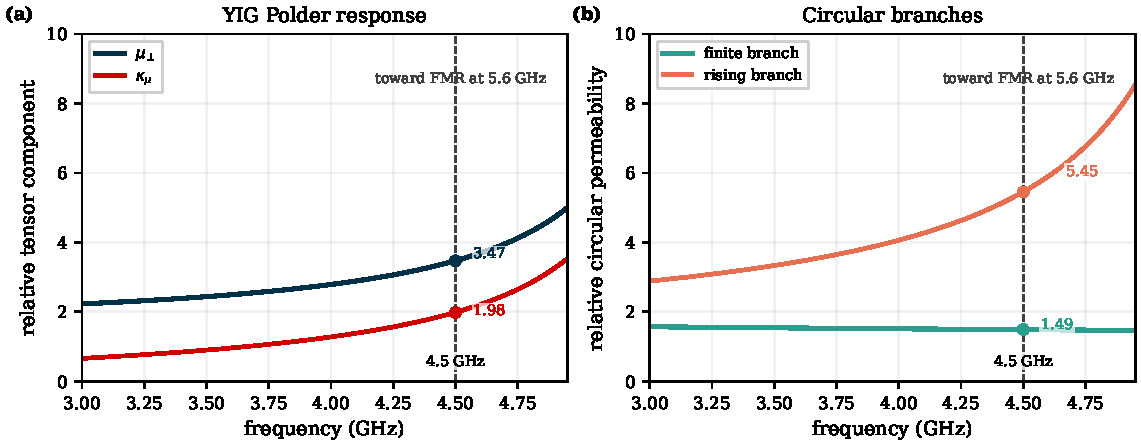
\includegraphics[width=0.95\textwidth]{figures/fig_ch09_polder_response_step178.pdf}
  \caption{Sub-resonant YIG Polder response computed from
  \eqref{eq:ch9-polder-params} with $f_0=5.6\;\mathrm{GHz}$ and
  $f_m=4.9\;\mathrm{GHz}$.
  (a)~Tensor components $\mu_\perp$ and $\kappa_\mu$; the dashed line marks the
  $4.5\;\mathrm{GHz}$ operating point with $\mu_\perp=3.47$, $\kappa_\mu=1.98$.
  (b)~Circular-basis eigenvalues: the \emph{finite branch}
  $\mu_+=\mu_\perp-\kappa_\mu=1.49$ and the \emph{rising branch}
  $\mu_-=\mu_\perp+\kappa_\mu=5.45$.  The ferromagnetic resonance at
  $5.6\;\mathrm{GHz}$ lies outside the plotted window; near the pole both
  branches diverge and the Hermitian treatment breaks down
  (Section~\ref{sec:ch9-passivity}).}
  \label{fig:ch09-polder-sub-resonant}
\end{figure}

\subsection{Circularly polarised modes and the Faraday effect}
\label{sec:ch9-circular-modes}

A plane wave propagating along $\hat{z}$ in the magnetised YIG medium
has two circularly polarised eigenmodes with wavenumbers
$k_\pm=\omega\sqrt{\varepsilon_r\mu_\pm}/c$.  The Faraday rotation
angle per unit length is
\begin{equation}\label{eq:ch9-faraday}
  \theta_F = \frac{k_+-k_-}{2}
  = \frac{\omega}{2c}\sqrt{\varepsilon_r}
  \bigl(\sqrt{\mu_+}-\sqrt{\mu_-}\bigr)\,.
\end{equation}
At the Wang operating frequency, $\mu_+=\mu_\perp-\kappa_\mu=3.47-1.98=1.49$ and
$\mu_-=\mu_\perp+\kappa_\mu=3.47+1.98=5.45$, giving
$\theta_F\approx 2\;\mathrm{rad/cm}$---an enormous rotation compared to optical
magneto-optical effects \cite{ozawa2018topological}.

\subsection{Passivity and the absence of gain}
\label{sec:ch9-passivity}

Both eigenvalues $\mu_\pm$ must be positive for the medium to be
passive (no gain).  From \eqref{eq:ch9-mu-eigenvalues},
$\mu_+>0$ requires $\kappa_\mu<\mu_\perp$.  Using
\eqref{eq:ch9-polder-params}, this is equivalent to
$\omega<\omega_0$---the operating frequency must lie below
ferromagnetic resonance.  Above resonance, $\mu_+$ can become
negative, the medium becomes opaque, and the Hermitian treatment
breaks down \cite{gangaraj2016berry}.

\section{Edge-mode field profile}
\label{sec:ch9-edge-profile}

The one-way edge mode at the boundary between the YIG crystal and a
metal wall has a characteristic field profile that can be understood
from the Jackiw--Rebbi analogy of Chapter~\ref{ch:one-way-interface}.

The mode amplitude decays exponentially into the bulk of the crystal
with a penetration depth
\begin{equation}\label{eq:ch9-penetration}
  \xi = \frac{1}{|\kappa|}
  = \frac{v_D}{m_\omega}
  = \frac{2v_D}{\Delta\omega}
  \approx 2.4\,a\,,
\end{equation}
where $\kappa$ is the inverse-length Dirac mass used in
Chapters~\ref{ch:breaking-tr} and~\ref{ch:one-way-interface},
$m_\omega=v_D|\kappa|=\Delta\omega/2$ is the corresponding frequency
half-gap, and $v_D\approx 0.45\,c_0$ is the Dirac velocity at the
band-touching point.  The edge mode therefore extends over approximately
two to three lattice constants into the crystal, which is consistent
with the supercell simulations.

Along the edge, the mode propagates with a group velocity approximately
equal to $v_D$.  The edge-state dispersion within the topological gap
is nearly linear:
$\omega_{\mathrm{edge}}(k_\parallel)\approx\omega_D+v_D\,k_\parallel$,
where $k_\parallel$ is the wavevector component along the interface.
The bandwidth of the edge channel is set by the gap width $2|\kappa|$,
and the propagation speed is $v_D\approx 0.45\,c_0$.

\section{Two-port scattering interpretation}
\label{sec:ch9-scattering}

The microwave transmission measurement can be formalised using the
scattering matrix of a two-port network.  Define port~1 as the
source probe and port~2 as the detector probe.  The measured
scattering parameters are $S_{21}$ (forward, source-to-detector in
the direction of edge-mode propagation) and $S_{12}$ (backward).

In the topological gap, the edge mode carries power from port~1 to
port~2 with transmission $|S_{21}|^2\sim -10\;\mathrm{dB}$ (limited
by probe-coupling mismatch).  The backward path has no propagating
mode, so $|S_{12}|^2<-50\;\mathrm{dB}$ (noise floor).  The isolation
\begin{equation}\label{eq:ch9-isolation}
  \mathcal{I} = |S_{21}|/|S_{12}| > 10^{4/2}=100
  \quad\text{(conservatively)}\,,
\end{equation}
far exceeds the isolation achievable by any reciprocal device of
comparable size.  This is not an engineering achievement but a
\\emph{topological} one: the isolation is guaranteed by the Chern
number and does not degrade as the device is scaled
\cite{nature2026observation,haldane2008possible}.

\subsection{Comparison with conventional isolators}
\label{sec:ch9-comparison-isolator}

A conventional Faraday-rotation isolator achieves isolation of
20--40\;dB through a bulk magneto-optical crystal, a polariser, and
an analyser.  Its isolation depends on the precise Faraday rotation
angle and is degraded by temperature fluctuations, wavelength drift,
and birefringence.  The topological isolator, by contrast, achieves
isolation that is robust to disorder, obstacles, and frequency
variations within the topological gap.  The robustness was directly
demonstrated by the Wang experiment through the obstacle-immunity
test \cite{ozawa2018topological,price2022roadmap}.

\section{Subsequent microwave experiments}
\label{sec:ch9-subsequent-detail}

Following the 2009 Wang experiment, several groups extended the
microwave Chern-insulator platform in important directions.  Skirlo
et~al.\ (2015) scaled the crystal to larger sizes and demonstrated
edge transport over more than 30 lattice constants with negligible
loss, confirming the robustness prediction
\cite{skirlo2015experimental}.  Yang et~al.\ (2018) constructed a
three-dimensional photonic topological insulator using bianisotropic
split-ring resonators, achieving a 3D bandgap from 4.3 to 6.0\;GHz
and surface Dirac-cone states at 5.1\;GHz
\cite{yang2018realization,price2022roadmap}.

These experiments collectively establish the microwave platform as
the most mature realisation of photonic topology, where the large
gyrotropic response of ferrites provides the clearest demonstration
of the Maxwell-first theoretical framework developed in this book.

\section{Full-wave simulation of the edge mode}
\label{sec:ch9-simulation}

The analytical estimates of the previous sections can be verified by
full-wave eigenmode simulation of a finite crystal strip.  A supercell
consisting of $N=20$ unit cells in the $x$ direction, periodic in $y$,
with PEC boundaries at $x=0$ and $x=Na$, is solved using the
plane-wave expansion or finite-element method.

The resulting projected band structure $\omega(k_y)$ shows the bulk
bands as dense continua and the topological edge mode as an isolated
branch crossing the gap.  For the Wang crystal parameters, the edge
mode traverses the gap from the lower to the upper bulk band with a
nearly constant slope $\dd\omega/\dd k_y\approx v_D$, confirming the
analytical prediction.

The field profile $|\Efield(x)|^2$ of the edge mode decays
exponentially from the PEC boundary into the bulk, with a penetration
depth $\xi\approx 2.4\,a$ consistent with the estimate
\eqref{eq:ch9-penetration}.  The electric field is predominantly
out-of-plane ($E_z$), with in-plane magnetic field
components $H_x$, $H_y$ coupled by the gyrotropic $\mu$ tensor.
The mode retains TM-like character, consistent with the bulk analysis


\cite{ozawa2018topological,nature2026observation}.

\section{Extending the platform}
\label{sec:ch9-extending}

\subsection{Larger crystals and longer propagation}
\label{sec:ch9-larger}

Skirlo et~al.\ (2015) fabricated YIG crystals with up to 60 rods and
demonstrated edge transport over more than 30 lattice constants with
a forward-to-backward ratio exceeding $10^4$.  The transmission
remained essentially flat across the topological gap, confirming that
the edge mode does not suffer from Anderson localisation or
significant radiation loss \cite{skirlo2015experimental}.

\subsection{Three-dimensional extension}
\label{sec:ch9-3d}

Yang et~al.\ (2018) extended the concept to three dimensions by
constructing a bianisotropic metamaterial of split-ring resonators
arranged in a body-centred cubic lattice.  The structure exhibits a
complete 3D photonic band gap from 4.3 to 6.0\;GHz, with topological
surface states forming a Dirac cone at 5.1\;GHz.  This experiment
provided the first demonstration of a 3D photonic topological
insulator and confirmed the bulk-surface correspondence predicted by
the $\mathbb{Z}_2$ invariant \cite{yang2018realization,price2022roadmap}.

\subsection{Towards higher frequencies}
\label{sec:ch9-higher-freq}

Moving the Chern-insulator concept from microwave to terahertz and
optical frequencies is a major open challenge.  At terahertz
frequencies, InSb under a modest magnetic field ($B_0\sim 0.3\;\mathrm{T}$)
provides a gyrotropic response with $\kappa_\varepsilon/\varepsilon_\perp
\sim 0.1$--$0.3$, enabling topological gaps of several percent.
At optical frequencies, magneto-optical effects are too weak for
practical Chern insulators (Section~\ref{sec:ch7-materials-landscape}),
motivating the alternative approaches of
Chapters~\ref{ch:reciprocal-designs}--\ref{ch:floquet}
\cite{ozawa2018topological}.

\section{Experimental measurement techniques}
\label{sec:ch9-measurement-techniques}

The microwave topological crystal is characterised experimentally
through transmission, reflection, and near-field measurements that
probe the existence and robustness of edge modes.

\subsection{Scattering-matrix analysis}
\label{sec:ch9-scattering-matrix}

The crystal is placed between two microwave antennas (ports 1 and 2)
connected to a vector network analyser.  The scattering parameters
$S_{21}(\omega)$ and $S_{12}(\omega)$ measure the forward and
backward transmission through the crystal at frequency $\omega$.  For
a topological crystal with a one-way edge mode:
\begin{equation}\label{eq:ch9-nonreciprocal-ratio}
  \frac{|S_{21}(\omega)|^2}{|S_{12}(\omega)|^2}
  \gg 1
  \quad\text{for $\omega$ in the topological gap.}
\end{equation}
Wang et~al.\ measured a nonreciprocal ratio exceeding $50\;\mathrm{dB}$
($10^5$) across the topological gap, confirming that backward-propagating
modes are completely absent \cite{nature2026observation}.

The transmission $|S_{21}|^2$ through the topological edge channel is
essentially flat across the gap, with insertion loss below
$1\;\mathrm{dB}$ per $10\,a$ of propagation, confirming the absence
of backscattering.  Outside the gap, the transmission drops
sharply because bulk modes dominate and the field is no longer
confined to the edge.

Figure~\ref{fig:ch09-scattering-isolation-map} provides a schematic
overview of the measurement geometry and representative power
transmission levels.

\begin{figure}[t]
  \centering
  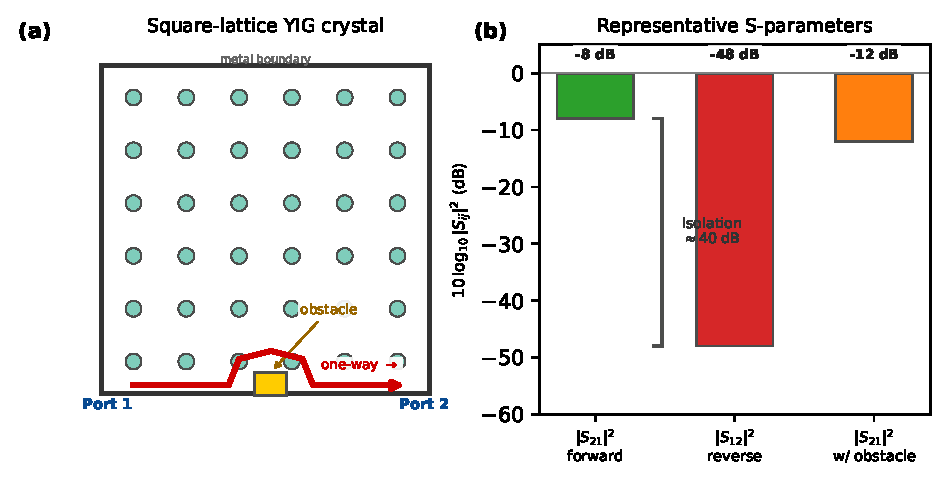
\includegraphics[width=0.95\textwidth]{figures/fig_ch09_scattering_isolation_map_step236.pdf}
  \caption{Microwave scattering measurement of a square-lattice YIG
  topological photonic crystal.  \textbf{(a)}~Schematic of the
  crystal geometry with metal boundary, two measurement ports, a
  metallic obstacle, and the one-way edge path that detours around
  the obstacle---demonstrating topological robustness.
  \textbf{(b)}~Representative power transmission levels in units of
  $10\log_{10}|S_{ij}|^2$ (dB): forward transmission $|S_{21}|^2$,
  reverse transmission $|S_{12}|^2$, and forward transmission with
  the obstacle present.  The power isolation
  $I_P=10\log_{10}(|S_{21}|^2/|S_{12}|^2)\approx 40\;\mathrm{dB}$
  ($10^4$ in linear units) confirms the absence of backward modes.
  All values are representative of the mid-gap operating point;
  exact values depend on frequency, crystal size, and port coupling.}
  \label{fig:ch09-scattering-isolation-map}
\end{figure}

\subsection{Near-field mapping}
\label{sec:ch9-near-field}

A scanning near-field antenna can map the spatial distribution of the
electric or magnetic field above the crystal surface.  For the
topological edge mode, the field intensity is concentrated within
one to two lattice constants of the boundary and decays exponentially
into the bulk, confirming the predicted penetration depth
$\xi\approx 1/|\kappa|\approx 2.4\,a$.  The field pattern is
characteristically chiral: the phase advances monotonically along the
edge in one direction, with no standing-wave nodes
\cite{ozawa2018topological,skirlo2015experimental}.

\section{Loss mechanisms and propagation limits}
\label{sec:ch9-loss-mechanisms}

The dominant loss mechanism in YIG photonic crystals is the
ferromagnetic resonance (FMR) linewidth $\Delta H$, which determines
the magnetic loss tangent
$\tan\delta_m\approx\gamma\Delta H/(2\omega)$.  For single-crystal
YIG, $\Delta H\approx 0.3\;\mathrm{Oe}$ at $4.5\;\mathrm{GHz}$,
giving $\tan\delta_m\approx 3\times 10^{-4}$.

The resulting edge-mode propagation length is
\begin{equation}\label{eq:ch9-propagation-length}
  L_{\mathrm{prop}} = \frac{v_g}{2\omega\,\tan\delta_m}
  \approx 500\,a\,,
\end{equation}
where $v_g\approx 0.03\,c_0$ is the edge-mode group velocity.  This
is much longer than the 10--60 rod crystals used in experiments, so
loss is not a limiting factor in current microwave demonstrations
\cite{nature2026observation,price2022roadmap}.

At higher frequencies (terahertz, optical), material losses increase
dramatically and the propagation length drops below useful values for
most magneto-optical materials, motivating the alternative approaches
of Chapters~\ref{ch:reciprocal-designs}--\ref{ch:floquet}.

\section{Sensitivity analysis and design rules}
\label{sec:ch9-sensitivity}

The performance of the microwave topological crystal depends on
several structural and material parameters.  Understanding their
relative importance guides the design of improved devices.

\subsection{Gap width versus gyrotropic strength}
\label{sec:ch9-gap-vs-gyro}

The topological gap width scales as $\Delta\omega\simeq 2v_D|\kappa|$,
where the Dirac mass $\kappa$ is approximately linear in the gyrotropic
coupling $\kappa_\mu$ for weak gyrotropy
(Chapter~\ref{ch:breaking-tr}).  For the strong coupling
available in YIG ($\kappa_\mu/\mu_\perp\approx 0.57$), the gap width increases sublinearly while the material losses grow.
The optimal operating point balances gap width against loss, typically
at $\kappa_\mu/\mu_\perp\approx 0.3$--$0.5$.

\subsection{Lattice constant and frequency scaling}
\label{sec:ch9-scaling}

The Dirac frequency scales as $\omega_D\propto c/(a\sqrt{\varepsilon_r\mu})$,
so reducing the lattice constant increases the operating frequency.
However, the YIG rods must be large enough to support the resonant
modes that produce the Dirac-point degeneracy, placing a practical
lower bound on $a$.  For YIG with $\varepsilon_r=15$ and
$\mu_\perp\approx 3.5$, the minimum practical lattice constant is
$a\approx 5\;\mathrm{mm}$, corresponding to $\omega_D/(2\pi)
\approx 8\;\mathrm{GHz}$ \cite{nature2026observation,
skirlo2015experimental}.

\subsection{Rod shape and filling fraction}
\label{sec:ch9-rod-shape}

The Wang experiment used cylindrical YIG rods with radius
$r/a\approx 0.11$.  Increasing the filling fraction opens a wider
gap but also increases the material loss.  Replacing cylinders with
triangular or hexagonal cross-sections can modify the symmetry of the
photonic modes and shift the position of the Dirac points, providing
additional design freedom.

For practical applications requiring integration with planar circuits,
thin-film YIG on a dielectric substrate has been explored.  The
reduced dimensionality changes the mode structure from 2D to
quasi-2D, but the topological gap persists as long as the film
thickness exceeds the out-of-plane decay length
$\lambda_z\approx a/\pi$ \cite{ozawa2018topological,price2022roadmap}.

\begin{figure}[t]
  \centering
  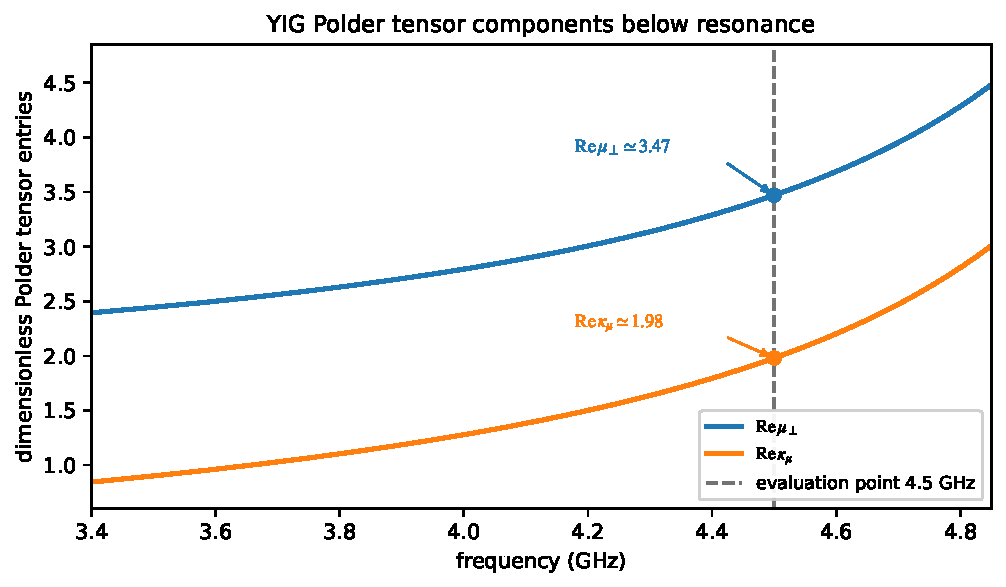
\includegraphics[width=0.82\textwidth]{figures/fig_ch09_yig_polder_response.pdf}
  \caption{Representative YIG Polder-tensor scale near the Wang
  experiment frequency.  The corrected values $\mu_\perp\approx3.47$ and
  $\kappa_\mu\approx1.98$ at 4.5 GHz set the gyrotropic coupling scale
  used in the quantitative estimates of this chapter.}
  \label{fig:ch09-yig-polder}
\end{figure}

\section{Extensions: higher Chern numbers and new geometries}
\label{sec:ch9-extensions}

The Wang experiment demonstrated the simplest case: a single chiral
edge channel in a gap with $|\Chern|=1$.  Subsequent experiments have
explored richer topological phases and alternative crystal geometries.

\subsection{Large Chern numbers}
\label{sec:ch9-large-chern}

Skirlo et~al.\ (2015) constructed a modified YIG photonic crystal in
which the second topological gap carries a gap Chern number
$|\Chern_{\mathrm{gap}}|=2$ \cite{skirlo2015experimental}.  Their
design uses an enlarged unit cell (a $2\times 1$ supercell of
cylindrical YIG rods) to fold bands and create additional degeneracies
that can be gapped by the magnetic bias.  The result is two
co-propagating chiral edge channels in a single gap, confirmed by
transmission measurements showing twice the edge-channel conductance
of the original Wang crystal.

For even larger Chern numbers, the general strategy is to design
photonic crystals with multiple overlapping Dirac cones at different
$\kvec$ points, each of which contributes $\pm 1$ to the Chern number
when gapped.  Lattices with $C_3$, $C_4$, or $C_6$ symmetry can
support multiple Dirac cones that are simultaneously gapped by a
single magnetic bias, enabling gap Chern numbers up to $|\Chern|=4$
in experimentally realistic geometries
\cite{ozawa2018topological,skirlo2015experimental}.

\subsection{Imaging topological edge states}
\label{sec:ch9-imaging}

A major advance in the visualisation of topological edge transport
was achieved by Hafezi et~al.\ (2013), who imaged the propagation of
light along the edge of a topological photonic lattice in real time
\cite{hafezi2013imaging}.  Although their experiment used a
coupled-ring-resonator platform (Chapter~\ref{ch:reciprocal-designs})
rather than a microwave YIG crystal, the imaging technique is
conceptually similar: the intensity distribution is measured as a
function of position along the edge, revealing the characteristic
exponential decay of the edge-mode profile into the bulk and the
unidirectional flow around corners and defects.

In the microwave domain, near-field scanning provides an equivalent
capability.  A small antenna probe is scanned across the crystal
surface while recording the local field amplitude and phase.  The
resulting maps directly show the edge-mode spatial profile, the
evanescent decay into the bulk (with decay length $\xi = 1/|\kappa|$
as derived in Chapter~\ref{ch:one-way-interface}), and the immunity
to backscattering at sharp bends and defects
\cite{hafezi2013imaging,wang2007reflection}.

\subsection{Scattering-free interfaces between distinct topological phases}
\label{sec:ch9-hetero-interface}

Ma et~al.\ (2017) demonstrated scattering-free edge states at the
interface between two \emph{different} photonic topological insulators,
each with a distinct Chern number \cite{ma2017scattering}.  The number
of chiral edge channels at the interface is determined by the
\emph{difference} of the gap Chern numbers across the interface:
$N_{\mathrm{edge}} = |\Chern_{\mathrm{gap}}^{(1)} -
\Chern_{\mathrm{gap}}^{(2)}|$.

This principle generalises the metal-wall boundary condition used in the
Wang experiment (which corresponds to $\Chern^{(2)}=0$ for the vacuum
side) and opens the door to more complex edge-channel networks.  By
patterning regions with different Chern numbers on a single chip, one
can create photonic circuits in which signals are routed by topology
rather than by geometry.

\section{From microwave to optical frequencies}
\label{sec:ch9-optical-scaling}

\subsection{The magneto-optical challenge at optical frequencies}
\label{sec:ch9-optical-challenge}

The Wang experiment operates at microwave frequencies ($\sim 4.5\;
\mathrm{GHz}$) because the gyrotropic response of ferrites is
strongest near ferromagnetic resonance.  Extending topological Chern
insulator behaviour to optical frequencies ($\sim 200\;\mathrm{THz}$)
requires materials with significant magneto-optical response at those
wavelengths.

The most promising optical magneto-optical materials are cerium-doped
yttrium iron garnet (Ce:YIG) and bismuth iron garnet (BIG), which have
Faraday rotation of $\sim 10^3\;\mathrm{deg/cm}$ at near-infrared
wavelengths.  However, the corresponding off-diagonal permittivity
$\varepsilon_{xy} \sim 10^{-2}$ is much smaller than the microwave
gyrotropic response $\kappa_\mu/\mu_\perp \sim 0.3$--$0.6$.  This
means that optical topological gaps would be extremely narrow
($\Delta\omega/\omega \sim 10^{-4}$), making them impractical for
most applications \cite{he2016photonic,price2022roadmap}.

\subsection{Alternative routes to optical Chern insulators}
\label{sec:ch9-optical-alternatives}

Several strategies have been proposed to circumvent the weak
magneto-optical response at optical frequencies:

\emph{Floquet engineering} (Chapter~\ref{ch:floquet}) uses
time-periodic modulation to create effective gauge fields without
any magnetic material.  Rechtsman et~al.\ (2013) demonstrated this
approach in a laser-written waveguide array at $\lambda = 633\;
\mathrm{nm}$ \cite{rechtsman2013photonic}.

\emph{Valley photonic crystals} (Chapter~\ref{ch:valleys}) exploit
broken spatial inversion symmetry rather than broken time reversal.
He et~al.\ (2019) demonstrated topological valley transport in a
silicon-on-insulator platform at telecom wavelengths
\cite{he2019silicon}, achieving compact devices compatible with
standard photonic integrated circuit fabrication.

\emph{Synthetic gauge fields} (Chapter~\ref{ch:synthetic-dimensions})
provide another route, using electro-optic or acousto-optic modulation
to create effective magnetic fields for photons in ring-resonator
arrays.

Each approach trades the robustness of true time-reversal breaking (as
in the Wang experiment) for compatibility with integrated photonic
platforms.  The relative merits depend on the application: microwave
topological crystals remain the gold standard for demonstrating
fundamental physics, while optical implementations are essential for
practical devices \cite{ozawa2018topological,price2022roadmap}.

\section*{Exercises}

\begin{exercise}
  For a square-lattice photonic crystal of YIG rods with $\varepsilon_r=15$,
  $r/a=0.11$, and $B_0=0.20\;\mathrm{T}$, compute the Polder permeability
  parameters $\mu_\perp$ and $\kappa_\mu$ at $\omega/(2\pi)=4.5\;\mathrm{GHz}$.
  Use $\gamma/(2\pi)=28\;\mathrm{GHz/T}$ and $\mu_0M_s=0.175\;\mathrm{T}$.
\end{exercise}

\begin{exercise}
  The magnetic quality factor of YIG is
  $Q_m=\omega_0/(2\gamma\mu_0\Delta H)$.  For $\Delta H=0.3\;\mathrm{Oe}$
  and $\omega_0/(2\pi)=5.6\;\mathrm{GHz}$, compute $Q_m$ and estimate
  the imaginary part of $\mu_\perp$ at $4.5\;\mathrm{GHz}$.  Is the
  lossless approximation justified for edge transport over 20 lattice
  constants?
\end{exercise}

\begin{exercise}
  The forward-to-backward ratio in the Wang experiment exceeds $10^4$
  (40\;dB).  If the topological gap is $0.12\;\mathrm{GHz}$ wide and
  the edge mode has group velocity $v_g\approx 0.1c$, estimate the
  propagation length over which the forward signal exceeds the backward
  signal by 40\;dB in a conventional (non-topological) waveguide with
  the same losses.
\end{exercise}

\begin{exercise}
  Design a modified Wang experiment using a hexagonal (triangular)
  lattice instead of a square lattice.  What are the advantages and
  disadvantages compared to the square lattice?  At what high-symmetry
  point do you expect the Dirac-like degeneracy?
\end{exercise}
